\section{Materials and Methods}

\subsection{Experiments}
A total of 23 right-handed subjects took part in the experiment (9 females, 14 males, $24 \pm 4.6$ years old). All subjects were non-smokers and without respiration problems. According to their self-reports, none had a history of injury in the olfactory bulb or incapability of smelling. Subjects were informed about the experimental protocol and the purpose of the study. None of the participants in experiment were wearing perfumed products on the day of experiment. 

10 different odors were provided for the experiment, including rose water, lavender oil, jasmine oil, chocolate powder, mint oil, valerian pills, garlic powder, star anise, rotten cooked cauliflower and baby shampoo. The odorants were placed inside covered bottles so as to avoid effects of their visual characteristics.

After the set up of the EEG recording system, subjects were asked to relax and close their eyes. One odor bottle was randomly selected and provided to the subject's nostrils at 1-2 cm. The subjects were not informed about the name of the odor during the experiment. The same odor was presented for about 15 times, leading to about 15 trials. Each trial consisted of 6 seconds baseline and 6 seconds odor experience. After experiencing an odor, the subjects were asked to rate it in terms of pleasantness, using a 5-point Linkert scale that ranged from very unpleasant to very pleasant. 
%More details about the experiment can be found in~\cite{kroupi2014non}.     

Regarding the equipment, an EGI's Geodesic EEG system (GES) 300 was used to record, amplify and digitalize the EEG signals. EEG signals were recorded from a 256-channel EEG Net Amps 300 cap with sampling frequency of 250Hz.  

\subsection{Pre-processing of EEG Signals}
After the pre-cleaning and synchronization of recorded EEG signals by GES-300 system, a total of 12 seconds EEG segment is kept for each trial. It contains 6 seconds of baseline (resting state) and 6 seconds of activity (odour perception). Signals from 40 electrodes which locate on face muscles and around eyes are rejected in order to reduce muscle and eye movement artifacts. Signals from the remaining 216 electrodes are kept for further analysis. 

A bandpass filter (4th order butterworth) is applied for the EEG signals with pass-band 0-50Hz. Small laplacian filter is applied for each electrode in order to reduce volume conduction effects~\cite{wolters2007volume}. Remaining Eye-movement artifacts are rejected manually by using Independent Component Analysis (funcitons are provided by EEGLAB\copyright~ toolbox~\cite{luck2014introduction}). Topographic maps of ICA components are plotted for each trial, components showing strong activities around eye-region are examined and rejected if their statistics confirms that they are artifact components~\cite{luck2014introduction}. The number of components removed depends varies for each trial of each subject. 

\subsection{Construction of Functional Connectivity Networks}
Functional connectivity can be estimated in various ways. Two time-doman functional connectivity models were applied and compared in this paper, which are Linear Granger Causality model~\cite{roebroeck2005mapping}  and Nonlinear Regression Analysis model~\cite{bettus2008enhanced}. We applied both models to our 216-channel EEG signals and the performances of estimated functional connectivity networks were analysed by feature extraction and classification on pleasantness during olfactory perception. The details of how to estimate functional connectivity networks by using these two models are described below.

\subsubsection{Linear Granger Causality}
Granger causality is first proposed by C.W.J. Granger in investigating causal relations in econometric models in 1969~\cite{granger1969investigating}. Decades later this concept is introduced into various neurophysiological studies. It is used to measure the causality between activities in different neuron assemblies, which estimates the functional connectivity over brain regions. 

Suppose we have two time series $X_t$ and $Y_t$. Let $U_t$ denote all the information accumulated from both time series since time $t-1$, and $U_t-Y_t$ denotes all this information apart from the specified series $Y_t$. $\sigma^2(X|U)$ is the variance of $\epsilon_t(X|U)$, in which $\epsilon_t(X|U)=X_t-P_t(X|U)$ and $P_t(X|U)$ represents the optimal, unbiased, least-squares predictor of $X$ using the set of values $U$.

\emph{Definition of Causality}: If $\sigma^2(X|U)<\sigma^2(X|\overline{U-Y})$, then Y is causing X, denoted by $Y_t \Rightarrow X_t$. Under the notion of Granger causality, $Y_t$ is causing $X_t$ if $X_t$ is better predicted using all available information than if the information from $Y_t$ is excluded.

The definition of Granger causality represents a theoretic approach which is difficult to implement due to lack of knowledge of the distributions of the estimators. In order to solve this problem, different approaches for computing Granger causality have been developed. In this paper we use the Vector Auto-Regression model (VAR)~\cite{barnett2014mvgc} to estimate Granger causality since it provides better computational efficiency and numerical accuracy~\cite{barnett2014mvgc}. 

According to the VAR model, we suppose signals from two channels (i.e., two electrodes in our case) are $\mathbf{X_t}$ and $\mathbf{Y_t}$. Then
\begin{equation} \label{eq:GC}
\mathbf{U_t} =  \begin{pmatrix}
                  \mathbf{X_t}\\
                  \mathbf{Y_t}
                \end{pmatrix} = \sum_{k=1}^{p} \begin{pmatrix}
                                                  A_{xx,k} & A_{xy,k}\\
                                                  A_{yx,k} & A_{yy,k}
                                                \end{pmatrix} \begin{pmatrix}
                                                              \mathbf{X_{t-k}}\\
                                                              \mathbf{Y_{t-k}}
                                                                    \end{pmatrix} + \begin{pmatrix}
                                                                                      \mathbf{\epsilon_{x,t}}\\
                                                                                      \mathbf{\epsilon_{y,t}}
                                                                                    \end{pmatrix}
\end{equation}
\\
$U_t$ represents the combined time series by $X_t$ and $Y_t$, which will be used in VAR model for regression and analysis of dependence between $X_t$ and $Y_t$. The residuals covariance matrix $\Sigma$ from the residual terms in \eqref{eq:GC} is estimated as
\begin{equation}
\Sigma \equiv cov \begin{pmatrix}
                   \mathbf{\epsilon_{x,t}}\\                                                                             \mathbf{\epsilon_{y,t}}
                  \end{pmatrix} = \begin{pmatrix}
                                   \Sigma_{xx} & \Sigma_{xy}\\                                                                           \Sigma_{yx} & \Sigma_{yy}
                                  \end{pmatrix}.
\end{equation}

In this paper we use the MVGC toolbox~\cite{barnett2014mvgc} to estimate the parameters in the VAR model. We first estimate the best model order \emph{p} by using the AIC (Akaike Information Criterion). The minimum model order is selected by using a regression model of Morf's version of the LWR (the initials stand for Levinson, Whittle, Wiggins and Robinson) algorithm~\cite{morf1978recursive}. Similarly to the estimation of the model order, the LWR is also used for estimating the VAR parameters. The Granger causality from $\mathbf{Y_t}$ to $\mathbf{X_t}$ is then defined as:
\begin{equation} \label{eq:GC_F}
F_{\mathbf{Y_t}\rightarrow \mathbf{X_t}} \equiv ln \frac{|\Sigma_{xx}'|}{|\Sigma_{xx}|}.
\end{equation}
In Equation \eqref{eq:GC_F}, $|\Sigma_{xx}'|$ represents the covariance matrix of the reduced regression (the regression contains only $\mathbf{X_t}$, and $\mathbf{X_t}$ is predicted only by information from its own past), while $|\Sigma_{xx}|$ represents the covariance matrix of the full regression (which contains both $\mathbf{Y_t}$ and $\mathbf{X_t}$). Thus, the value of $F$ provides the "amount of information" transmitted from $\mathbf{Y_t}$ to $\mathbf{X_t}$ by estimating the reduction in the prediction error when $\mathbf{Y_t}$ is included in the prediction of $\mathbf{X_t}$. When there is no information transmitted from $\mathbf{Y_t}$ to $\mathbf{X_t}$ (i.e., $|\Sigma_{xx}'|=|\Sigma_{xx}|$), then $F=0$. There is no upper limit on the values of $F$.

\subsubsection{Nonlinear Regression Analysis}
Nonlinear regression analysis is also a commonly used way to estimate the functional connectivity, which is represented by statistical coupling between EEG signals. This method is introduced by Pijin and Lopes Da Silva for EEG analysis~\cite{pijn1990localization}. Nonlinear regression analysis can quantify the relationships between different EEG signals in order to determine whether activity in one neuron assembly depends on that of other assemblies.
\begin{figure}[!t]
    \centering
    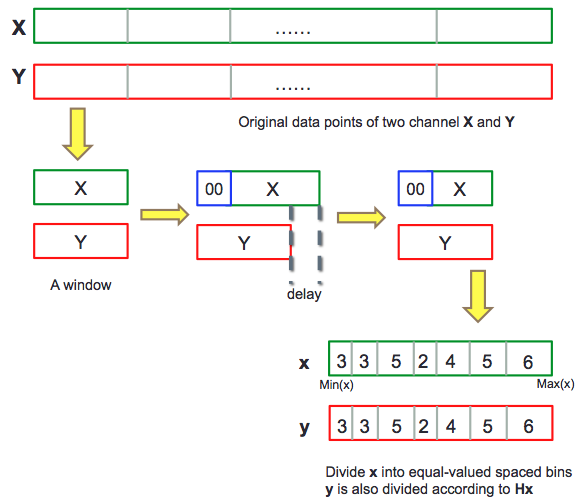
\includegraphics[width=0.45\textwidth]{./images/binsepa.png}
    \caption{An example of separating EEG time series into windows and bins for computing the nonlinear regression curves}
    \label{fig:bin}
\end{figure}
Suppose we have two channels of EEG signals $x$ and $y$, then nonlinear regression analysis provides a measure called \emph{correlation ratio} $\eta^2$, whose estimator is called $h^2$. $\eta^2$ (or $h^2$) gives a statistical measure that describes the dependency of signal $x$ on $y$. Assume the amplitude of signal $y$ is a function of the amplitude of signal $x$. The expectation of $y$ given a value of $x$ is denoted as $\mu_{y|x}$ where:
\begin{equation} \label{eq:regressioncurve}
\mu_{y|x} = \int_{-\infty}^{\infty} y p(y|x) \mathrm{d}y,
\end{equation}
and $\mu_{y|x}$ describes the predicted value of $y$ given $x$. By this definition, we can calculate $\eta^2$, which represents the reduction of variance of $y$ that obtained by predicting $y$ value using $\mu_{y|x}$. $\eta^2$ is expressed as:
\begin{equation} \label{eq:NRAregression}
\eta^2 = \frac{Total \ Variance - Unexplained \ Variance}{Total \ Variance}
\end{equation}
Explained variance is the variance calculated from $y$ according to $\mu_{y|x}$. In this paper, the nonlinear regression analysis algorithm is implemented by fieldtrip toolbox\copyright~\cite{oostenveld2010fieldtrip}. the procedure is depicted in Fig. \ref{fig:bin}).

\subsection{Significance Check}
The significance check is similar for both methods (Grancer causality and Nonlinear Regression Analysis) and is split into two main parts: (1) $p$-value calculation for samples based on theoretical asymptotic null distribution; (2) statistical significance adjusted for \emph{Bonferroni} correction. The rationale behind applying a significance check is to keep only the significant connections. 

The \emph{null hypothesis} $H_0$ is set to "there is no functional connectivity between two channels". In this paper, we assume that the connectivity values emanate from a normal distribution and the $p$-value that rejects the null hypothesis is set to $p=0.05$. The commonly used $F$-statistics is applied for estimating the $p$-value both for Granger Causality and for Nonlinear Regression Analysis.

All the values in functional connectivity maps that passed significance check are kept for feature extraction and classification in later steps. In order to keep the information about the strength of the connections, we use weighted maps. The weights emanate from the original values of the functional connectivity maps (estimated either with Granger causality or with nonlinear regression analysis) that survived the significance check (an example is presented in Fig. \ref{fig:weightednetwork}).

%\begin{Fig.}[!t]
%    \centering
%    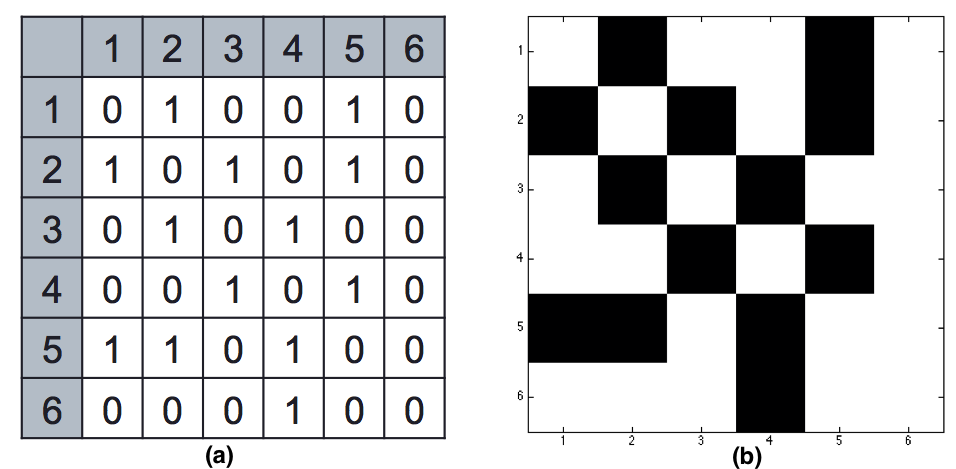
\includegraphics[width=0.45\textwidth]{./images/unweightednetwork.png}
%    \caption{An example of unweighted functional connectivity map construction of size $6 \times 6$. Nodes in (a) with value 1 represents the nodes that passed significance check. (b) is a visual expression of unweighted functional connectivity map.}
%    \label{fig:unweightednetwork}
%\end{Fig.}

\begin{figure}[t]
\centering
%\mbox{
	\leavevmode
\subfigure[]{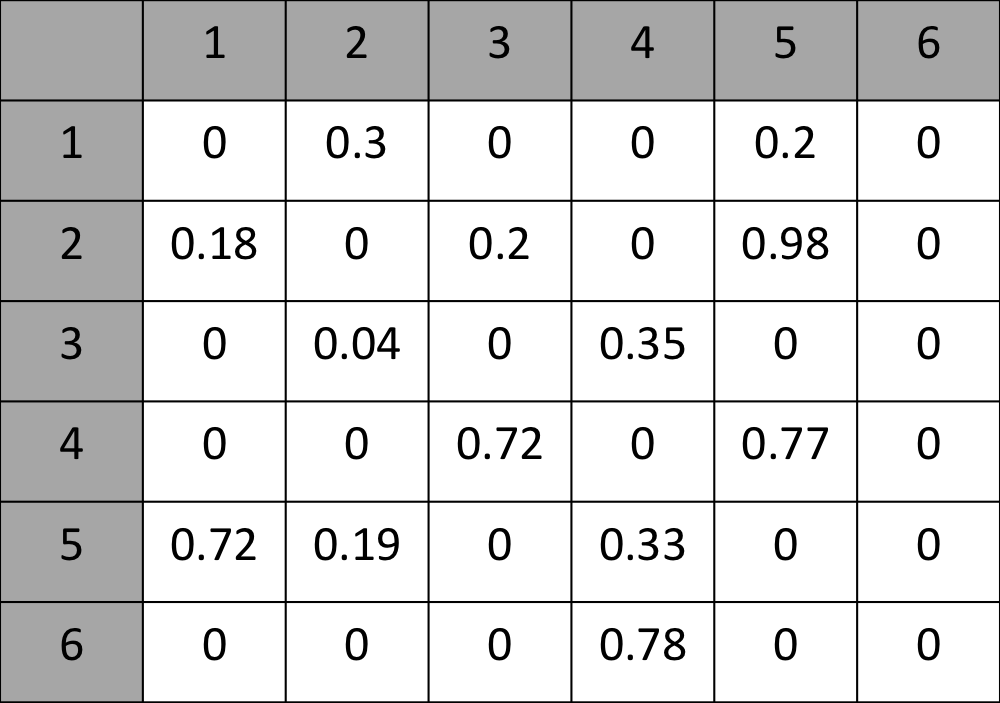
\includegraphics[width=0.48\linewidth]{images/weighted_fcm0.png}}
\subfigure[]{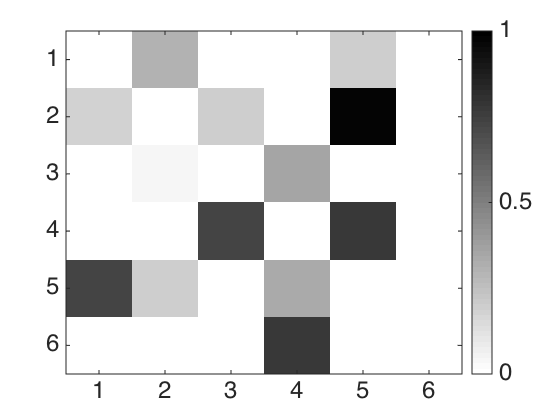
\includegraphics[width=0.48\linewidth]{images/weighted_fcp.png}}
%}
\caption{An example of a weighted functional connectivity map of size $6 \times 6$. In (a) the values represent the weights of the nodes. Each weight corresponds to the value of the underlying functional connectivity map. (b) A visual presentation of the same weighted functional connectivity map.}\label{fig:weightednetwork}
\end{figure}

%\begin{figure}[!t]
%    \centering
%    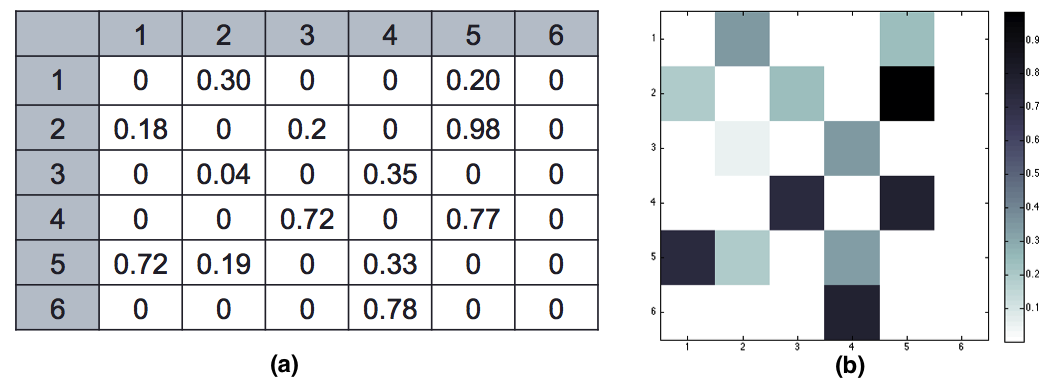
\includegraphics[width=0.45\textwidth]{./images/weightednetwork.png}
%    \caption{An example of a weighted functional connectivity map of size $6 \times 6$. In (a) the values represent the weights of the nodes. Each weight corresponds to the value of the underlying functional connectivity map. (b) A visual presentation of the same weighted functional connectivity map.}
%    \label{fig:weightednetwork}
%\end{figure}

\subsection{Network Feature Extraction}
The functional connectivity maps give us a view of how channels communicate information with each other, thus we can consider this map as a network. Different ways of treating brain networks have been proposed by different groups. For instance, some research groups see the brain as a scale-free network~\cite{eguiluz2005scale}, while others view it as a small-world network~\cite{bassett2006small}. In this section, we introduce two categories of network features, based on the principles of scale-free networks and of small-world networks, namely -- \emph{physical statistics} features for scale-free networks, and \emph{graph theory-based} features for small-world networks.

\subsubsection{Small-World Network Features}
A small-world network consists of nodes that can be reached from every other node with a small number of steps. Different aspects of small-world networks have been studied and here, based on the commonly used features in neural network studies, we introduce four features for analysing the functional connectivity maps which are \emph{characteristic path}, \emph{global efficiency}, \emph{local efficiency} and \emph{clustering coefficient}~\cite{watts1998collective}~\cite{latora2001efficient}.

\emph{Characteristic path} represents the average shortest path of the network. The minimum value is achieved when the network is a complete graph (every pair of distinct vertices is connected by a unique edge). In our case, we can interpret the characteristic path as a feature representing the number of connections in the functional connectivity networks. The more the connections in the functional connectivity network, the smaller the value of the characteristic path, thus the faster the information that is transferred through the network. 

The concept of \emph{global efficiency} of a small-world network is introduced by Latora and Marchiori~\cite{latora2001efficient} and provides a measure of efficient behaviour of the network, by assuming that the network system is parallel (i.e., every vertex sends information concurrently through its edges in the network). The global efficiency of the network is higher when the characteristic path is short. Thus, global efficiency measures how efficiently the vertices exchange information through the network concurrently. Similarly with global efficiency, \emph{local efficiency} is defined as the average efficiency of the subgraphs of the neighbours of a vertex $i$ in the graph (details of computing subgraphs can be referred to~\cite{ullmann1976algorithm}). The subgraphs of $i$ do not contain vertex $i$, hence, the local efficiency can show how efficient the communication is when $i$ is removed from the network. Thus the local efficiency reveals how much the network is fault tolerant. 

Finally, \emph{clustering coefficient} of a network measures the degree to which vertices in a graph tend to cluster together. The overall level of clustering in a network is given by Watts and Strogatz~\cite{watts1998collective} as the average of the local clustering coefficients of all vertices. 

\subsubsection{Scale-Free Network Features}
Although graph theory has been successfully used to describe brain functional connectivity networks, a few studies have shown that brain functional connectivity can also be considered as a scale-free network. An example of a scale-free compared to a random network is presented in Fig. \ref{fig:scalefree}. The number of links $k$ of a node in a scale-free network follows a power law distribution as \eqref{eq:pwlaw}.
\begin{equation} \label{eq:pwlaw}
P(a \ node \ having \ k \ links ) \sim k^{-\lambda}
\end{equation}
where $\lambda$ is a parameter valued in the range $2<\lambda<3$.
Groups of CJ Stam~\cite{stam2004functional} have found that brain functional connectivity network can be viewed as a scale-free network because the connectivity distribution followed a power-law scaling with an exponent close to two.
%, which suggests such functional connectivity network can be considered as a scale-free network topology~\cite{van2008small}. Detailed analysis can also be found in Thivierge's work~\cite{thivierge2014scale}.

\begin{figure}[!t]
    \centering
    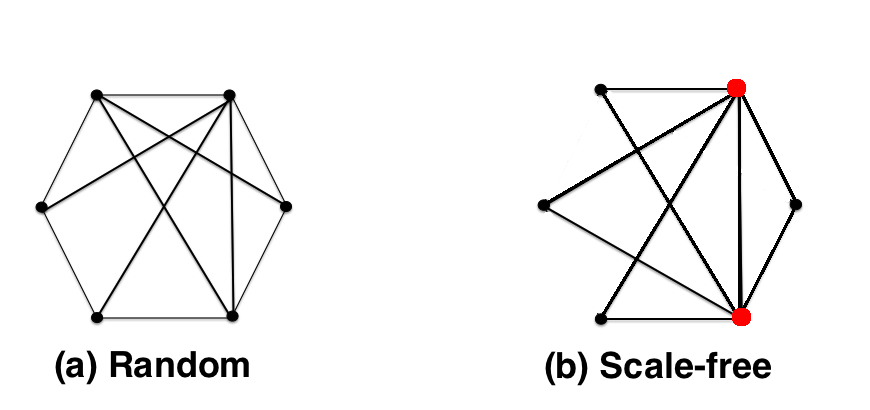
\includegraphics[width=0.4\textwidth]{./images/Scale-free.png}
    \caption{An example of a random network (a) compared with a scale-free network (b) . Red nodes in (b) represent the hubs holding connections in the subgraph.}
    \label{fig:scalefree}
\end{figure}

In information theory, \emph{entropy} plays an important role in measuring uncertainty. Recently, following theoretical and statistical mechanics paradigms, several entropy measures for complexity have been proposed for network structures, and these measures have shown good performance in quantifying the level of organisation encoded in structural features of scale-free networks. It is well known that \emph{Shannon entropy} and \emph{von Neumann entropy} are related to the information present in classical and quantum systems respectively. Both of them can be used to analyse the structural organisation of scale-free networks\cite{anand2009entropy}. 

The amount of \emph{Shannon entropy} has a correlation with the number of network structural constraints. Examples of network constrains include: a) fixed number of links per vertex, b) given degree sequence (a monotonic non-increasing sequence of the degrees of vertices in the graph), and c) community structure (vertices of the network can be easily grouped into sets of vertices such that each set of vertices is densely connected internally). From this point of view, we can conclude that Shannon entropy has a clear interpretation of quantifying the information presented in network structure (Detailed proof can be referred to~\cite{anand2009entropy}). If a network has a smaller Shannon entropy, it will have more constrains on its structure, which shows this network is more optimal. 

\emph{Von Neumann entropy} has been defined by von Neumann for proving the irreversibility of quantum measurement processes. Recently it is also shown that von Neumann entropy can also be applied to network analysis~\cite{passerini2008neumann}. It has been shown that von Neumann entropy is a measure of regularity of networks~\cite{passerini2008neumann}. For a fixed number of edges, regular networks (networks whose vertices have the same number of neighbours) have in general a higher von Neumann entropy. It is also shown that von Neumann entropy depends on the number of connected components, long paths and nontrivial symmetries. With a fixed number of edges, von Neumann entropy is smaller for networks with higher degree of cluster. The mathematical proofs can be found in~\cite{passerini2008neumann} and~\cite{anand2009entropy}.

Thus, to sum up, network-based features including characteristic path, local efficiency, global efficiency, clustering coefficient, Shannon entropy and von Neumann entropy are extracted from the estimated functional connectivity maps for classification purposes. 

\subsection{Classification}

Support vector machine with a \emph{Gaussian radial basis function} kernel is used for classification. The parameter selection of $\sigma$ in RBF kernel is based on cross-validation. In particular, the dataset is split into three parts, namely training, validation and testing. Leave-one-subject-out (LOO) cross-validation is carried out to estimate the parameter $\sigma$. The testing is also carried out in a LOO cross-validation scheme. We tested 13 different values of parameter $\sigma$ ranged from 0.01 to 2. More specifically, the parameter $\sigma$ is selected based on the training and validation using data from 22 subjects, while one subject is left out for testing. The procedure is repeated until all subjects have been left out as test-subjects (i.e., the procedure is repeated 23 times). 

Cohen's Kappa $\kappa$~\cite{uebersax1987diversity}, is a measure of agreement between two viewers, and is calculated to evaluate the classifier's performance. 
%Some researchers consider that Cohen's kappa can be used to evaluate the agreement by chance, i.e. if the viewers are randomly guessing for a decision. 
In our case the two viewers actually correspond to the ground truth and test labels. Cohen's kappa is considered an accurate metric for classification performance and takes into account unbalanced classes (i.e., classes with different number of samples). 
